\section{Benchmark}\label{sec:benchmark}
\frame{\tableofcontents[currentsection]}

% What libraries are used
\begin{frame}
\frametitle{Benchmark}
\begin{itemize}
\item Benchmarked libraries (most recent release):
\begin{itemize}
    \item \href{http://www.met.reading.ac.uk/clouds/adept/}{Adept 2.0.8}~\cite{hogan:2014}
    \item \href{https://github.com/coin-or/ADOL-C}{ADOL-C 2.7.2}~\cite{griewank:1996}
    \item \href{https://coin-or.github.io/CppAD/doc/cppad.htm}{CppAD 20200000}~\cite{bell:2020}
    \item \href{https://github.com/JamesYang007/FastAD}{FastAD 3.1.0}
    \item \href{https://github.com/trilinos/Trilinos/tree/master/packages/sacado}{Sacado 13.0.0}~\cite{phipps:2009}
    \item \href{https://github.com/stan-dev/math}{Stan Math Library 3.3.0}~\cite{carpenter:2015}
\end{itemize}
\item Used by others~\cite{carpenter:2015}\cite{margossian:2018}\cite{hogan:2014}.
\item Micro and macro-benchmarks.
\end{itemize}
\end{frame}

% Sum
\begin{frame}
\frametitle{Sum}

\begin{figure*}
    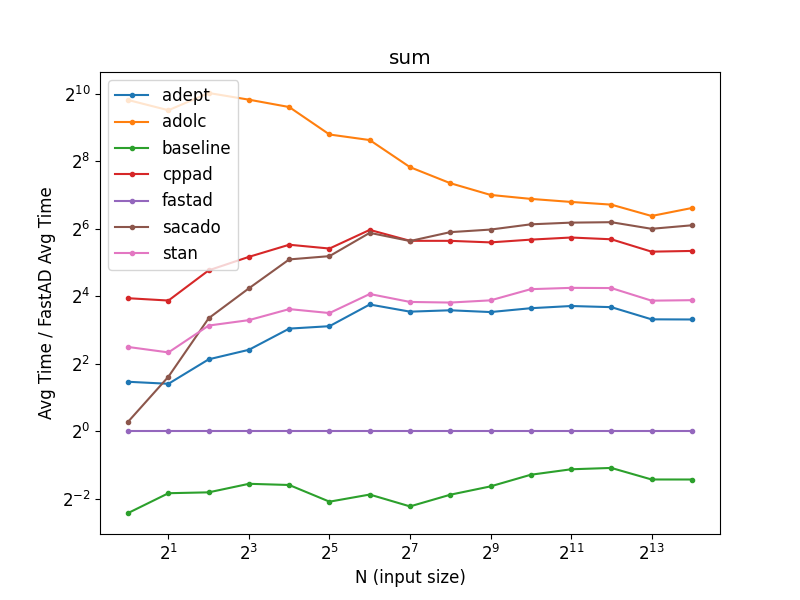
\includegraphics[width=0.7\textwidth]{../../figs/sum_fig.png}
\end{figure*}
    
\end{frame}

% Sum Iter
\begin{frame}
\frametitle{Sum Iterated}

\begin{figure*}
    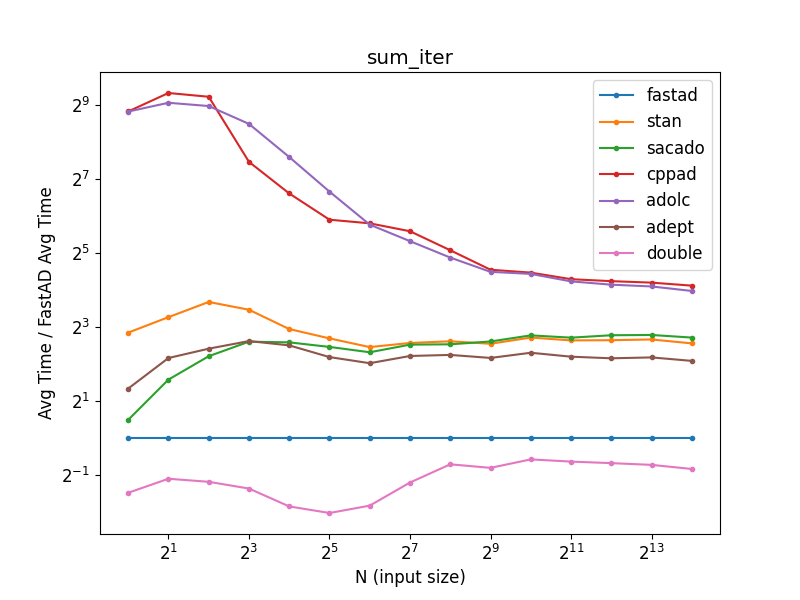
\includegraphics[width=0.7\textwidth]{../../figs/sum_iter_fig.png}
\end{figure*}
    
\end{frame}

% Log-Sum-Exp
\begin{frame}
\frametitle{Log-Sum-Exp}
\begin{figure*}
    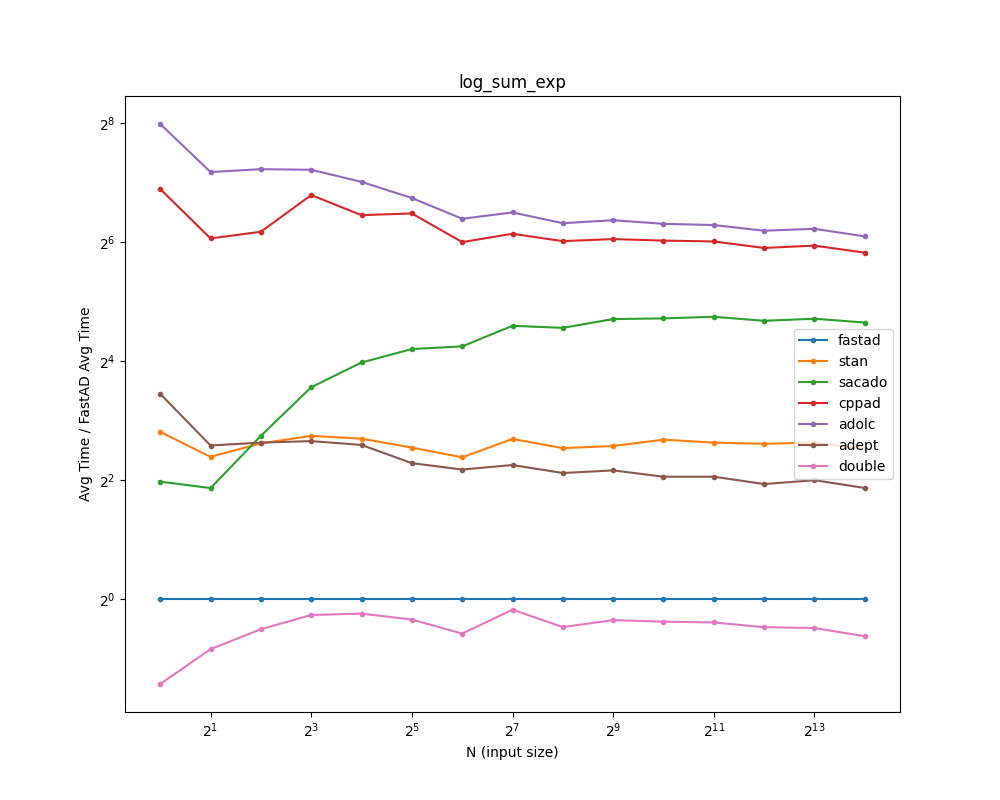
\includegraphics[width=0.7\textwidth]{../../figs/log_sum_exp_fig.png}
\end{figure*}
\end{frame}

% Matrix Multiplication
\begin{frame}
\frametitle{Matrix Multiplication + Summation}
\begin{figure*}
    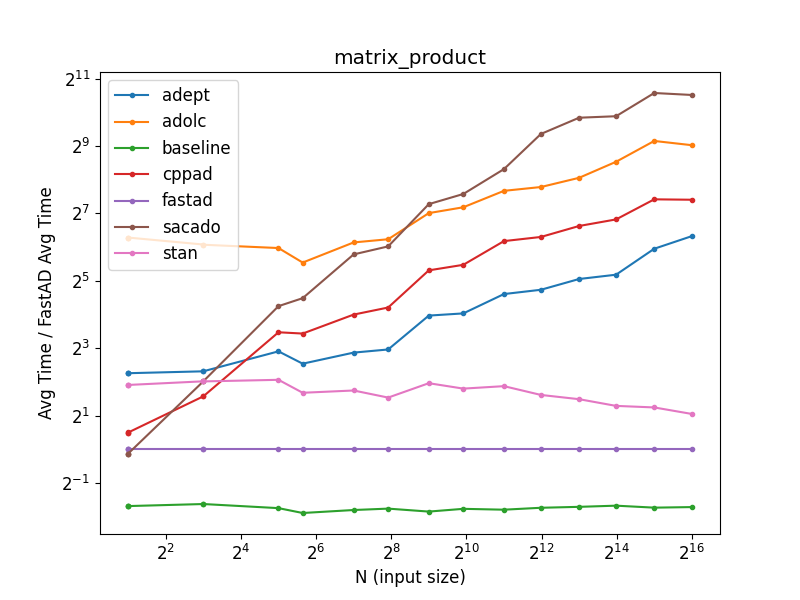
\includegraphics[width=0.7\textwidth]{../../figs/matrix_product_fig.png}
\end{figure*}
\end{frame}

\begin{frame}
\frametitle{Matrix Multiplication + Summation}
\begin{itemize}

\item FastAD/Baseline $= 3.14$.
\item Forward-eval: one multiplication of two $K\times K$ matrices.
\item Backward-eval: two multiplications of the same order.
    \begin{align*}
        \frac{\partial f}{\partial A} 
        &= \frac{\partial f}{\partial (A\cdot B)} \cdot B^T \\
        \frac{\partial f}{\partial B} 
        &= A^T \cdot \frac{\partial f}{\partial (A\cdot B)}
    \end{align*}
\item Total: three $K\times K$ matrix multiplications.
\item Manually-written gradient $\approx 3 * \text{Baseline}$.
\item FastAD / Manual $\approx \frac{3.14}{3} = 1.0475$.
\item $ 4.75\%$ overhead from manual!

\end{itemize}
\end{frame}

% Normal-lpdf
\begin{frame}
\frametitle{Normal Log-PDF}
\begin{figure*}
    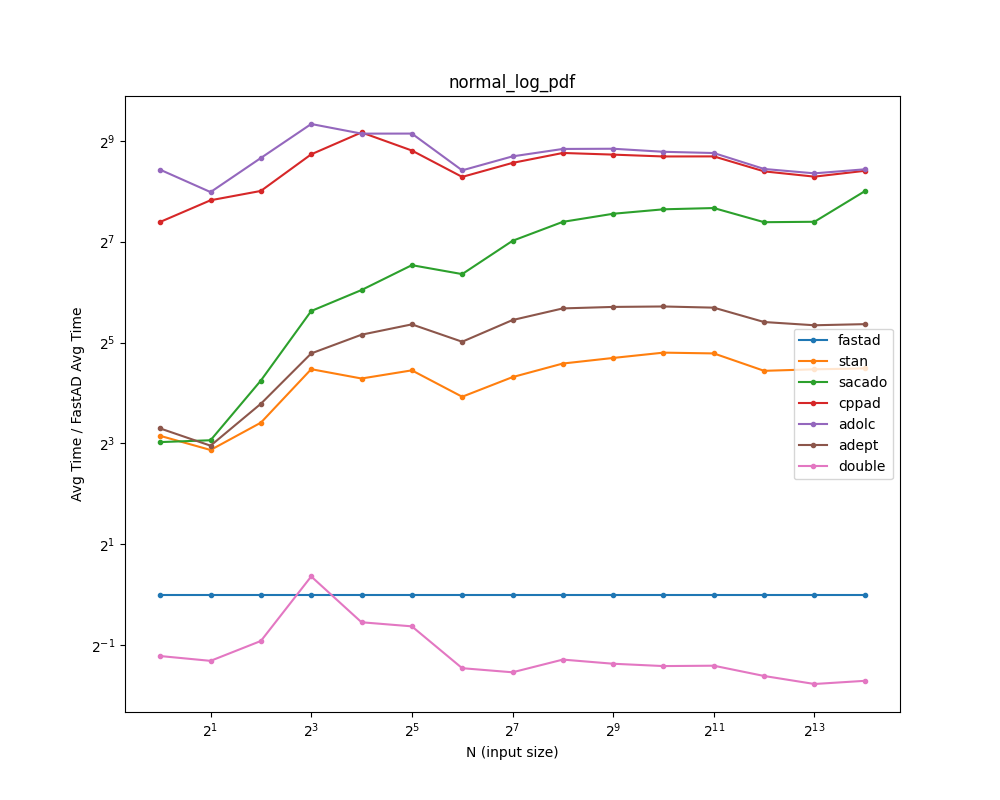
\includegraphics[width=0.7\textwidth]{../../figs/normal_log_pdf_fig.png}
\end{figure*}
\end{frame}

% Regression
\begin{frame}
\frametitle{Bayesian Regression Model}
\begin{align*}
    y &\sim N\paren{X\cdot w + b, \sigma^2} \\
    w &\sim N\paren{0,I} \\
    b &\sim N\paren{0,1} \\
    \sigma &\sim Unif\paren{0.1, 10.}
\end{align*}
\end{frame}

\begin{frame}
\frametitle{Bayesian Regression Model}
\begin{figure*}
    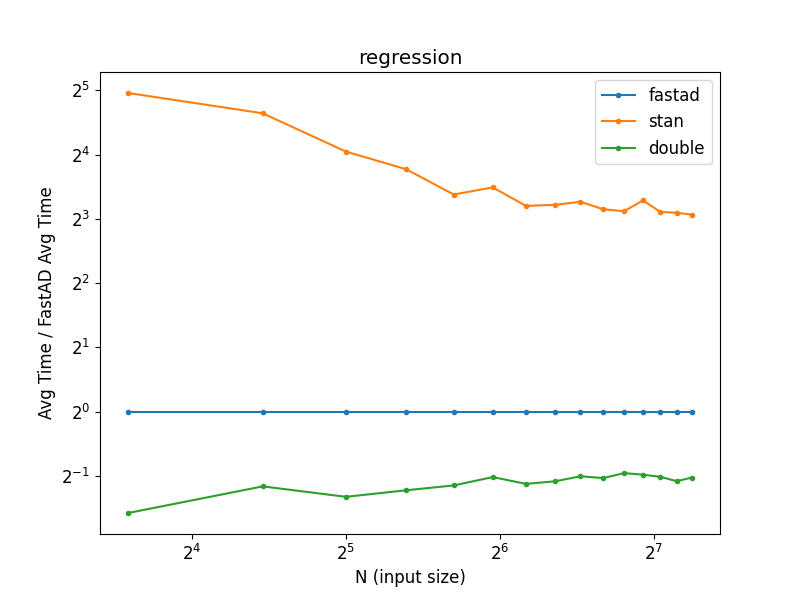
\includegraphics[width=0.7\textwidth]{../../figs/regression_fig.png}
\end{figure*}
\end{frame}

% Stochastic Volatility
\begin{frame}
\frametitle{Stochastic Volatility Model~\cite{stan-rm:2018}}
{\small
\begin{align*}
    y &\sim N(0, e^{h}) \\
    h_{std} &\sim N(0, 1) \\
    \sigma &\sim Cauchy(0,5) \\
    \mu &\sim Cauchy(0,10) \\
    \phi &\sim Unif(-1, 1) \\
    h &= h_{std} \cdot \sigma \\
    h[0] &= \frac{h[0]}{\sqrt{1 - \phi^2}} \\
    h &= h + \mu \\
    h[i] &= \phi \cdot (h[i-1] - \mu),\, i > 0
\end{align*}
}%
\end{frame}

\begin{frame}
\frametitle{Stochastic Volatility Model}
\begin{figure*}
    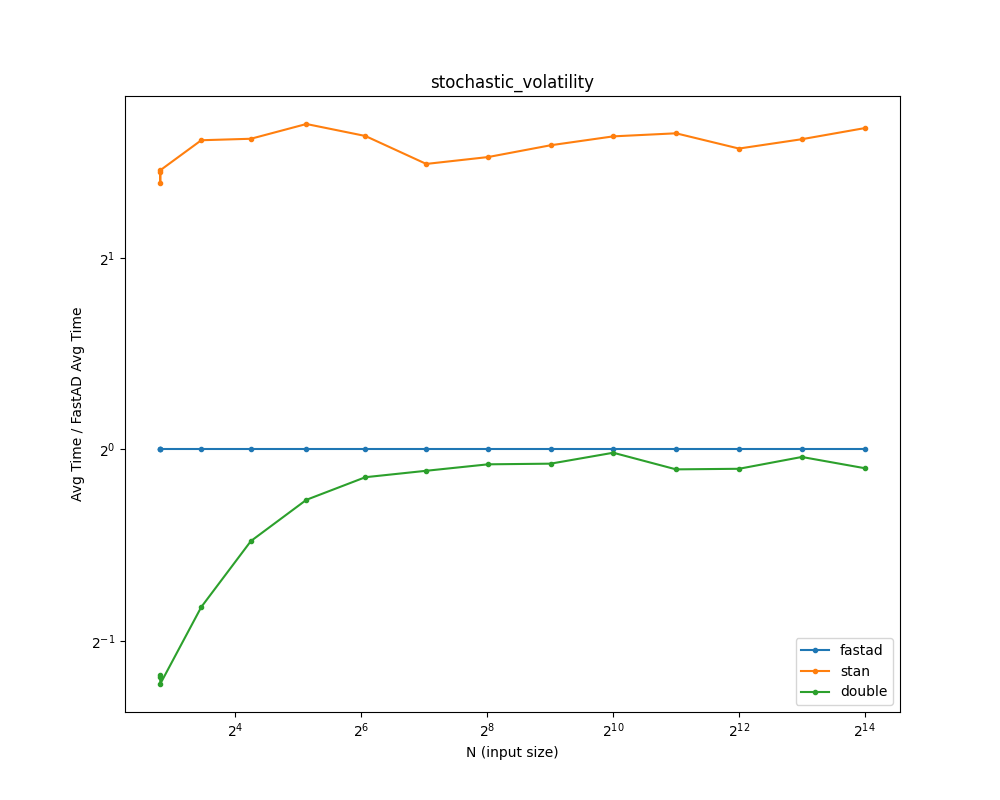
\includegraphics[width=0.7\textwidth]{../../figs/stochastic_volatility_fig.png}
\end{figure*}
\end{frame}

\begin{frame}
\frametitle{Stochastic Volatility Model}
\begin{itemize}
    
\item FastAD/baseline $= 1.24$
\item $24\%$ overhead from one \emph{forward-evaluation}.
\item Gradient computation is very cheap.

\end{itemize}
\end{frame}

% AutoPPL
\begin{frame}
\frametitle{Applications}
\begin{itemize}
    
\item How does FastAD perform in other applications?
\item Currently developing a PPL called \textbf{AutoPPL} using FastAD.\@
\item Similar to Stan, but all in C++.
\item We show a comparison of the regression model using NUTS
    between Stan and AutoPPL.\@

\end{itemize}
\end{frame}

\begin{frame}
\frametitle{Bayesian Regression Model}
\begin{figure*}
    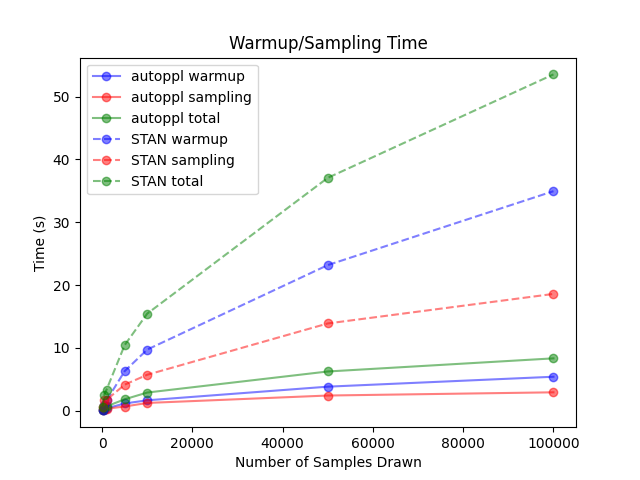
\includegraphics[width=0.7\textwidth]{figs/runtime.png}
\end{figure*}
\end{frame}

\begin{frame}
\frametitle{Bayesian Regression Model}
\begin{figure*}
    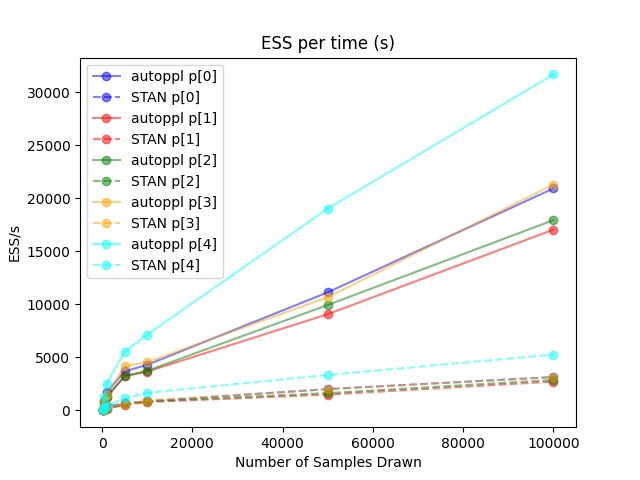
\includegraphics[width=0.7\textwidth]{figs/ess_s.png}
\end{figure*}
\end{frame}
